\documentclass[twocolumn]{article}

\usepackage{amsmath}
\usepackage{amssymb}
\usepackage{booktabs}
\usepackage{multicol}

\usepackage{tikz}
\usetikzlibrary{graphs,graphs.standard}


\usepackage{fancyhdr}

\pagestyle{fancy}
\fancyhf{}
\rhead{Problem Questions}
\lhead{Week \thepage}
\rfoot{Mathematics and Problem Solving 2021-22}

\begin{document}

\section{Formal Systems}

\subsection{}

    A formal system has states $A_1, \dots, A_5$ and rules $R$. Below is a graph showing all possible transitions between states.

    \begin{figure}[h!]
        \centering
        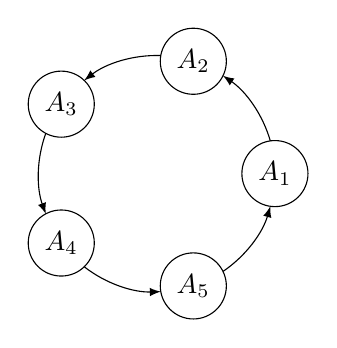
\begin{tikzpicture}

            \def \n {5}
            \def \radius {1.5cm}
            \def \margin {16} % margin in angles, depends on the radius
            
            \foreach \s in {1,...,\n}
            {
              \node[draw, circle] at ({360/\n * (\s - 1)}:\radius) {$A_\s$};
              \draw[->, >=latex] ({360/\n * (\s - 1)+\margin}:\radius) 
                arc ({360/\n * (\s - 1)+\margin}:{360/\n * (\s)-\margin}:\radius);
            }
            \end{tikzpicture}
    \end{figure}

    \begin{enumerate}
        \item Is the derivation $A_1 \Rightarrow^*_R A_5$ possible within this system?
        \item If so, provide a derivation.
    \end{enumerate}

\subsection{}

    A formal system has states $X_1, \dots, X_{7}$. The rules $R$ are such that from a state $X_i$ it is possible to derive the state $X_{i+1}$

    \begin{enumerate}
        \item List the steps in the derivation $X_1 \Rightarrow^*_R X_7$
        \item What is the length of this derivation?
        \item Is there a derivation $X_4 \Rightarrow^*_R X_3$?
    \end{enumerate}

\subsection{}

    A string rewriting system has the following rules $R$.

    \begin{itemize}
        \item $aba \curvearrowright b$
        \item $aaa \curvearrowright $
    \end{itemize}

    Let A be the string $aaaababbbbabababaaaababa$

    \begin{enumerate}
        \item List all the strings B that can be derived from A in one step: $A \Rightarrow_R B$
        \item List the strings in one possible derivation of T, $A \Rightarrow^*_R T$, where T is a terminal state (where no further rule applications are possible)
    \end{enumerate}

\subsection{}

    A string rewriting system is defined with the following rules.

    \begin{multicols}{2}
    \begin{itemize}
        \item $(fof) \curvearrowright f$
        \item $(fot) \curvearrowright t$
        \item $(tof) \curvearrowright t$
        \item $(tot) \curvearrowright t$
    \end{itemize}
\end{multicols}

    For each of the following, derive a terminal string (where no further rule applications are possible)

    \begin{enumerate}
        \item $((fot)ot)$
        \item $((fof)o(tot))$
        \item $(((tof)of)o(fo(fof)))$
        \item Give a string from which the string $f$ is derivable by a derivation of length 3
    \end{enumerate}

\subsection{}

    For the following binary relations, state whether they are: Reflexive, Symmetric, Transitive

    \begin{enumerate}
        \item $=$
        \item $ > $
        \item $ \leq $
        \item $ \ne $
        \item older than
        \item can be rotated (by some angle) to get
    \end{enumerate}

\subsection{}

    For the following table of binary operators, state whether they are: Commutative, Associative

    \begin{enumerate}
        \item $ + $
        \item $ \times $
        \item $ \div $
        \item $ \times \pmod{n} $
        \item $ \div \pmod{n} $
    \end{enumerate}   


\clearpage
\section{Modular Arithmetic}

\subsection{}

    Solve the following modular arithmetic questions

    \begin{enumerate}
        \item $(13 \mod 3) + (23 \mod 4)$
        \item $(22 \mod 7) \times (13 \mod 7)$
        \item $(14 \mod 55 + 42 \mod 55) \times (13 \mod 55)$
        \item $11 \div 7 \pmod{13}$
        \item $4 \div 11 \pmod{17}$
    \end{enumerate}

\subsection{}

    For each number below, give its modular inverse (if defined) under a modulus of 8

    \begin{multicols}{2}
    \begin{enumerate}
        \item $ 0^{-1} \pmod{8} $
        \item $ 1^{-1} \pmod{8} $
        \item $ 2^{-1} \pmod{8} $
        \item $ 3^{-1} \pmod{8} $
        \item $ 4^{-1} \pmod{8} $
        \item $ 5^{-1} \pmod{8} $
        \item $ 6^{-1} \pmod{8} $
        \item $ 7^{-1} \pmod{8} $
    \end{enumerate}
\end{multicols}

\subsection{}

    If multiplication distributes over subtraction under modulus then, which of the following statements are true

    \begin{enumerate}
        \item $a ( b - c ) \equiv a - bc \pmod{n} $
        \item $a ( b - c ) \equiv ab - ac \pmod{n} $
        \item $a ( b - c ) \equiv ac - ab \pmod{n} $
        \item $a - bc \equiv ab - ac \pmod{n} $
    \end{enumerate}

\subsection{}

    What is the additive inverse of:

    \begin{enumerate}
        \item $24$
        \item $5 \pmod{17}$
        \item $a \mod b$ (give your answer as a formula)
    \end{enumerate}

\subsection{}

    Write the following as products of their prime factors in the form $ f_1 \times f_2 \times f_3 \times \dots $

    \begin{multicols}{2}
        \begin{enumerate}
            \item $68$
            \item $123$
            \item $92$
            \item $44$
        \end{enumerate}
    \end{multicols}

\subsection{}

    Assume a string is encrypted using the encryption function $E(X) = (aX + b) \mod n$, where $X$ is the index of an element drawn from the alphabet [abcdefghijklmnopqrstuvwxyz0123456789], and $n$ is the length of that alphabet.

    \begin{enumerate}
        \item Encrypt the string ``hello'' with keys a=7, b=4
        \item Decrypt the string ``q4zajep'' with the same keys
    \end{enumerate}

\subsection{}

    Assume $p = 23$, $g = 7$. Alice generates a public key $A = 11$ using the following formula: $A = g^a \mod p$, where $A$ is the public key and $a$ is a private key.

    \begin{enumerate}
        \item Find a value for Alice’s private key by brute force
        \item You pick a private key $b = 11$. Calculate your public key, $B = g^b \mod p$
        \item A shared secret $s$ can be calculated with the formula $s = A^b \mod p$, where $A$ is Alice’s public key, and $b$ is your private key. Find $s$.
    \end{enumerate}

\subsection{}

    The following strings have been encrypted using the function $E(X_i) = (X + k + i) \mod 26$, where $i$ is the 1-based index of the character in the word to encrypt (ignoring spaces). For each, give a value for $k$.

    \begin{enumerate}
        \item ``kxbcqph'' (The first letter of plaintext is `c' )
        \item ``lacn ep gs'' (The plaintext is a sentence)
    \end{enumerate}

\subsection{}

VCKIVHH GSV UFMXGRLM FHVW GL VMXIBKG GSRH GVCG FHRMT Z ULINFOZ

\clearpage
\section{Number Systems}

\subsection{}

    Convert all the following values into each of: Binary, Octal, Decimal, and Hexadecimal

    \begin{enumerate}
        \item $ ( 01100011 )_2 $
        \item $ ( 0257)_8 $
        \item $ ( 611 )_{10} $
        \item $ ( 19\text{F} )_{16} $
    \end{enumerate}

\subsection{}

    Answer the following binary arithmetic questions. All numbers given are in binary. Representations use the number of bits shown. Give your answers in binary.

    \begin{enumerate}
        \item $0101011 + 1101011$
        \item $1101 - 1011$
        \item $00010100 - 10101000$
        \item $1101 \times 1010$
        \item $11101001 \times 00101001$
        \item $01001011 \div 00010111$ (report both quotient and remainder)
        \item $1011\div 0101$ (report both quotient and remainder)
    \end{enumerate}

\subsection{}

    Give the Two’s Complement for each of the following 8-bit binary numbers
        
    \begin{enumerate}
        \item 10000000
        \item 10100111
        \item 01101011
    \end{enumerate}

\subsection{}

    Calculate the answers to the following, working with 8-bit signed binary numbers \textbf{stored as sign and magnitude}

    \begin{enumerate}
        \item What is the additive inverse of $01101111$?
        \item $00110001 + 11001101$
        \item $10010101 - 00101010$
    \end{enumerate}

\subsection{}

   Give the greatest common divisor for each of the following pairs of numbers.

  \begin{enumerate}
       \item $(3, 7)$
       \item $(14, 39)$
       \item $(11, 23)$
   \end{enumerate}

\subsection{}

    What is the radix complement of the following numbers (assuming representation with the number of digits shown)?

    \begin{enumerate}
        \item $(52342)_{10}$
        \item $(00231)_{4}$
        \item $(01\text{FA})_{16}$
    \end{enumerate}

\subsection{}

    Assume base 32 is written with the alphabet [0-9A-V] Convert $(321223123212)_4$ into base 32

\subsection{}

    A 23 digit number in base 536 can store how many different values?

\subsection{}

    A web application needs to encode session ids in as few characters as possible. It can safely use numbers and upper and lowercase letters. What is the smallest number of characters that can encode the id 2348923947234?

\clearpage
\section{Sequences and Summation}

\subsection{}

    For each of the following, state whether the sequence is arithmetic or geometric, and give the next 3 values in the sequence

    \begin{enumerate}
        \item 1, 7, 13
        \item 0.9, 0.6, 0.4
        \item 2k, 6k, 18k
    \end{enumerate}

\subsection{}

    Give the first 5 elements of the following sequences:

    \begin{enumerate}
        \item $ \{ \frac{n^2}{n-1} \}^\infty_{n=1} $
        \item $ \{ i^3 \}^\infty_{i=3} $
        \item $ a_n = a_{n-1} + 3 $ where $a_1 = 22$
        \item $ a_n = 14 \times 3^{n-1} $
    \end{enumerate}

\subsection{}

    A geometric sequence has 10 terms and a common ratio of $\frac{1}{10}$ and it's final term is ${10^{-8}}$.

    \begin{enumerate}
        \item Is this sequence increasing, decreasing, monotonic, and/or bounded? (List all that apply)
        \item Is -10 a lower bound for this sequence?
        \item Is 1 an upper bound for this sequence?
    \end{enumerate}

\subsection{}

    Solve the following summations

    \begin{enumerate}
        \item $ \sum_{i=1}^{5} 2 $
        \item $ \sum_{i=4}^{7} i $
        \item $ \sum_{i=1}^{3} 2^i $
        \item $ \sum A $ where $ A = \{ n^2 \}^{7}_{n=1} $
    \end{enumerate}

\subsection{}

    Solve the following products

    \begin{enumerate}
        \item $ \prod_{k=1}^{3} (2k + 1) $
        \item $ \prod_{k=7}^{17} 2 $
        \item $ \prod A $ where $ A = \{ \frac{1}{k} \}^{4}_{k=1} $
    \end{enumerate}

\subsection{}

    Consider the sequence $S = \{ \frac{n}{n+1} \}^\infty_{n=1} $

    \begin{enumerate}
        \item Give a lower bound for this sequence that is also in this sequence.
        \item What is a number that this sequence will approach, but never quite reach?
        \item Is this sequence increasing, decreasing, monotonic, and/or bounded? (List all that apply)
    \end{enumerate}

\subsection{}

Simplify the following summations

\begin{enumerate}
    \item $ \sum_{i=1}^{n} c $
    \item $ \sum_{i=1}^{n} ( i + 2 ) $
    \item $ \sum_{i=1}^{n} ( i^2 + 3i ) $
    \item $ \sum_{i=1}^{n} \sum_{j=1}^{i} j $
    \item $ \sum_{i=1}^{n} A_i $ where $ A_n = A_{n-1} + \frac{1}{2} $ and $ A_1 = \frac{1}{2} $
\end{enumerate}


\clearpage
\section{Propositional Logic}

\subsection{}

When $p$ is true and $q$ is false, state whether the following statements are true or false

\begin{enumerate}
    \item $\neg \neg \neg q$
    \item $(p \wedge q) \vee p$
    \item $(p \vee \neg q) \implies p$
    \item $q \implies (p \Longleftrightarrow q)$
    \item $p \wedge q \Longleftrightarrow \neg p \vee q$
\end{enumerate}

\subsection{}

Let $p$ be a true proposition and $q$ be any proposition. Which of the following are true, and which of the following are false? (others might be true or false)

\begin{enumerate}
    \item $p \implies q$
    \item $q \implies p$
    \item $\neg q \implies p$
    \item $\neg p \implies q$
\end{enumerate}

\subsection{}

Construct a truth table for each of the following. For each, state whether the statement is always true, or if not give a case where it is false.

\begin{enumerate}
    \item $ p \implies (q \implies ( r \implies p )) $
    \item $ p \vee \neg r \implies (\neg ( r \wedge p ) $
\end{enumerate}

\subsection{}

Identify the atomic propositions in the following sentences and assign them each a letter (e.g. b = ``the bus is late'') Then express this as a statement of propositional logic using the notation taught in class

\begin{enumerate}
    \item If my bike is not working or the bus is late, then I am late for class
    \item I am happy if and only if I am riding my bike
\end{enumerate}

\subsection{}

For the following, state whether they are tautologies, contraditions, or contingiencies

\begin{enumerate}
    \item $p \implies (\neg p \vee p)$
    \item $p \vee q \implies p \wedge q$
    \item $\neg p \vee \neg\neg p$
    \item $p \vee \neg (p \vee \neg p) $
\end{enumerate}


\subsection{}

Do the following properties hold of implication? You may wish to use either a truth table or Equational Reasoning to arrive at your answer.

\begin{enumerate}
    \item Implication distributes over conjunction $$ (p \implies (q \wedge r)) \Longleftrightarrow (p \implies q) \wedge (p \implies r) $$
    \item Implication distributes over disjunction $$ (p \implies (q \vee r)) \Longleftrightarrow (p \implies q) \vee (p \implies r) $$
    \item Implication distributes over implication $$ (p \implies (q \implies r)) \Leftrightarrow (p \implies q) \implies (p \implies r) $$
\end{enumerate}

\subsection{}

Prove the following by Equational Reasoning. Format your proof as in the lecture slides

\begin{enumerate}
    \item $p \implies (p \vee \neg p)$
    \item $\neg p \wedge \text{true} \Longleftrightarrow \neg p$
\end{enumerate}

For this, use only the laws given in the lecture slides and the handout.


\clearpage
\section{Set Theory}

\subsection{}

    Define the following sets by extension

    \begin{enumerate}
        \item The set of natural numbers between 6 and 11 (not inclusive)
        \item The set of letters in the phrase ``formal systems, logic, and semantics''
        \item The set of sets with exactly one subset
    \end{enumerate}

\subsection{}

    State whether each of the following is a singleton, the empty set, or neither of these

    \begin{enumerate}
        \item The set of Real numbers, less the Natural numbers
        \item The set of even primes
        \item The set of digits used in binary
        \item The set black hearts in a standard deck of cards
        \item A set that has no proper subsets
        \item A set with exactly two subsets
    \end{enumerate}

\subsection{}

    Give the extension of the following sets

    \begin{enumerate}
        \item $\{ a, b, c \} \cap \{ c, d \} $
        \item $\{ a, c \} \cup \{ b, c, d \} $
        \item $\{ a, b, c \} \setminus \{ b, c, d \} $
        \item $\{ a \} \cap ( \{ b \} \cup \{a, b, c\} ) $
        \item $ (\{ c \} \cup \{ b \} \cup \{a\}) \cap ( \{b, c, a\} \cup \emptyset ) $
    \end{enumerate}

\subsection{}

    For the given sets, state whether the following propositions are true or false

    $ A = \{ a, b, c \} $

    $ B = \{ a, d \} $

    $ C = \{ c \} $

    \begin{enumerate}
        \item $ A \supset C $
        \item $ (C \cup A) \subseteq B $
        \item $ c \in ( A \cap B ) $
        \item $ a \not \in ( A \setminus B ) $
        \item $(B \cap \{d, a\} ) \supseteq B$
    \end{enumerate}

\subsection{}

    For the given sets, give the extension of the following sets

    $ A = \{ a, b, c \} $

    $ B = \{ a, d \} $

    $ C = \{ c \} $

    \begin{enumerate}
        \item $ (A \setminus B) \cap C$
        \item $ ( B \cap C ) \cup A $
        \item $ C \cup (A \setminus (B \cap A)) $
    \end{enumerate}

\subsection{}

Use equational reasoning to prove the following. Reference the laws of set theory and propositional logic introduced in the lectures and on the handout.

\begin{enumerate}
    \item $S \subseteq (T \cup (S \cap S)) $
    \item $ (S = T) \wedge (T \not\subseteq S) \Longleftrightarrow \text{false} $
    \item $ \emptyset \not\subset ((S \cap S) \setminus (S \setminus \emptyset)) $
\end{enumerate}

\clearpage
\section{Reading Week}
    

\clearpage
\section{Set Theory 2}

\subsection{}

    Give the cardinality of the following sets

    \begin{enumerate}
        \item $\{ 7, 8, 8\}$
        \item $\bigcap \{ \{ a, b \}, \{ b, a, d\}, \{d, f, a, b \}$ \}
        \item $\mathbb{P}(\{ a, b, c\})$
        \item $\mathbb{N}^0 \setminus \mathbb{N}^+$
        \item $\mathbb{Q} \setminus \mathbb{R}$
    \end{enumerate}

\subsection{}

    Give the cardinality of the following sets, given:

\begin{multicols}{2}
    \begin{itemize}
        \item $\#A = 4$
        \item $\#B = 6$
        \item $\mathbb{P}(C) = 8$
        \item $\#(A \cap B) = 1$
        \item $ C \subseteq A $
        \item $ \# (C \cap B) = \emptyset$
    \end{itemize}
\end{multicols}

    \begin{enumerate}
        \item $ A \cup B $
        \item $ \mathbb{P}(A \setminus B)$
        \item $ C \cap A $
        \item $ B \cup C $
        \item $ A \times B $
    \end{enumerate}

    \subsection{}

    Give the extension of the following sets.

    \begin{enumerate}
        \item $\mathbb{P}(\{ 1, 2, 3, 4 \})$
        \item $ \bigcup  \mathbb{P}(\{a, b, c\})  $
        \item $ \{a, b\} \times \{ a, b, c, d \} $
        \item $ \mathbb{P} ( \emptyset ) $
        \item $ \ ( \{ 1 \} \times \{ a, b \} ) \cap ( \{ 1, 2 \} \times \{ b, a \} ) $
    \end{enumerate}


\subsection{}

    Give the extension of the following sets.

    \begin{enumerate}
        \item $\{ n : \mathbb{N} \mid n \mod 3 = 1 \wedge n < 13 \} $
        \item $\{ n : \mathbb{N} \mid 4 < n < 7 \} $
        \item $ \{ n : \mathbb{N} \bullet n \mod 7 \} $
        \item $\{ a : \mathbb{R}; b : \mathbb{R}  \mid a^2 = b \wedge b^2 = a \bullet a \} $
        \item $\{ a : \mathbb{N}^+; b : \mathbb{N}^+  \mid a + b < 3 \bullet (a, b) \} $
    \end{enumerate}


\subsection{}

    Define by extension the set containing the smallest four elements of the following sets:

    \begin{enumerate}
        \item $ \{ n : \mathbb{N}^+ \bullet n^n \} $
        \item $ \{ n : \mathbb{N}^+ \bullet \frac{n}{n+1} \} $
    \end{enumerate}

\subsection{}

    Given the table below, give the extensions of the following sets

    \begin{table}[h!]
        \centering
        \begin{tabular}{c | c | c }
            \toprule
            Name & Age & Group \\
            \midrule
            Alice & 18 & A  \\
            Bob & 17 & B  \\
            Eve & 19 & A \\
            Mary & 22 & B \\
            \bottomrule
        \end{tabular}
    \end{table}

    \begin{enumerate}
        \item $ \{ x : Group \times Name \} $
        \item $ \{ x : Name \times Age \mid x.2 \ge 18 \bullet x.1 \} $
        \item $ \{ a : Name \times Group; b : Name \times Group \mid a.2 = b.2 \bullet \{a.1, b.1\} \} $
    \end{enumerate} 

\subsection{}

    For the table given above, define the following sets by set comprehension:

    \begin{enumerate}
        \item The set of all names
        \item The set of groups containing someone under the age of 18
    \end{enumerate}

\clearpage
\section{Graph Theory}

\subsection{}

    Consider the following graph.

    \begin{figure}[h!]
        \centering
    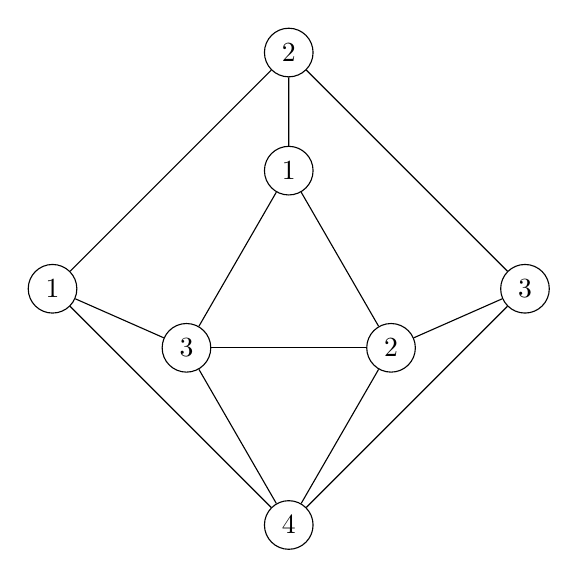
\begin{tikzpicture}
        \graph [simple, nodes={draw, circle, minimum size = .5cm}, clockwise] 
        {
          subgraph C_n [name=inner, radius = 1.5cm, n=3];
          subgraph C_n [name=outer, radius = 3cm, n=4];
        };
        \draw
         (inner 1) -- (outer 2)
         (inner 3) -- (outer 4)
         (inner 2) -- (outer 4)
         (inner 3) -- (outer 1)
         (inner 2) -- (outer 3);
        \end{tikzpicture}
    \end{figure}

    \begin{enumerate}
        \item Is it directed?
        \item Is it connected?
        \item Is it cyclic?
        \item What is the maximum degree of the graph?
        \item What is the degree of node 3?
        \item Create an adjacency matrix for the given graph
        \item List the loops in this graph as a set
    \end{enumerate}

\subsection{}

    A graph G is defined as $G = \{V, E\}$, where $V = \{ a, b, c \}$, and $E = V \times V$

    \begin{enumerate}
        \item Is it directed?
        \item Is it connected?
        \item Is it cyclic?
        \item What is the maximum degree of the graph?
        \item What is the degree of node b?
    \end{enumerate}

\subsection{}

    Below is a database for a social network

    \begin{table}[h!]
        \centering
        \begin{tabular}{c | c | c }
            \toprule
            Name & Age & Group \\
            \midrule
            Alice & 18 & A  \\
            Bob & 17 & B  \\
            Eve & 19 & A \\
            Mary & 22 & B \\
            \bottomrule
        \end{tabular}
    \end{table}

    A graph of connections is given by $ G = ( V, E)$ where $ V = \{ x : Name \}$, % and $ E = \{ x : Name \times Group; y : Name \times Group \mid x.2 = y.2 \bullet (x.1, y.1) \} $

    The graph has directed edges between those pairs of users who share a group

    \begin{enumerate}
        \item Give an extensional definition of E
        \item Give an intensional definition of E using set comprehension
    \end{enumerate}

\subsection{}

    A formal string-rewriting system is defined with the the rule $ a \rightsquigarrow abb $, and the starting string $a$.
    
    \begin{enumerate}
        \item Is $aaabbbbbb$ a string in this system? If so, draw a graph of the derivation $a \Rightarrow^* aaabbbbbb$
        \item Is there any derivation possible in this system that would result in a cyclic graph?
    \end{enumerate} 

\subsection{}

    A formal string-rewriting system is defined with the rules below. The starting string is $a$
    
    \begin{itemize}
        \item $ a \rightsquigarrow aba $
        \item $bab \rightsquigarrow b$
    \end{itemize} 

    \begin{enumerate}
        \item Draw a graph, of the first 5 unique strings that can be constructed in this system, where edges represent applications of one of the  grammatical rules
        \item Is this graph directed?
        \item Is this graph cyclic?
    \end{enumerate}

\clearpage
\section{Descriptive Statistics}

\subsection{}

    For the following types of data, say whether they are nominal, ordinal, or numeric, and give an appropriate measure of central tendancy to use to describe such data

    \begin{enumerate}
        \item Duration of daily commute
        \item Frequency in Hz
        \item DEFCON level
        \item Brands of espresso maker
    \end{enumerate}

\subsection{}

    For the following data, calculate the mean, median, and mode

    \begin{enumerate}
        \item 4, 2, 5, 2, 34, 2, 4
        \item 1, 4, 6, 2, 4, 3, 1
    \end{enumerate}

\subsection{}

    The following data represents a sample of scores collected from two levels of a mobile game. Calculate the range, inter-quartile range, and an appropriate form of standard deviation 

    \begin{enumerate}
        \item 1, 52, 3, 53, 23, 5, 3, 6
        \item 5, 2, 14, 25, 14, 11, 5
    \end{enumerate}

\subsection{}

    I recruit undergraduate students for a study on video game immersion, which is measured with a questionnaire. Half of the participants are asked to drink 3 cups of coffee before the experiment. Half are asked to not drink any coffee before the experiment.
    
    \begin{enumerate}
        \item What is my dependant variable?
        \item What is my independant variable?
        \item What is my sample?
    \end{enumerate}

\subsection{}

    What is the approximate correlation of the data shown? Pick the closest out of $\{-1, -0.5, 0, 0.5, 1\}$

    \begin{enumerate}
        \item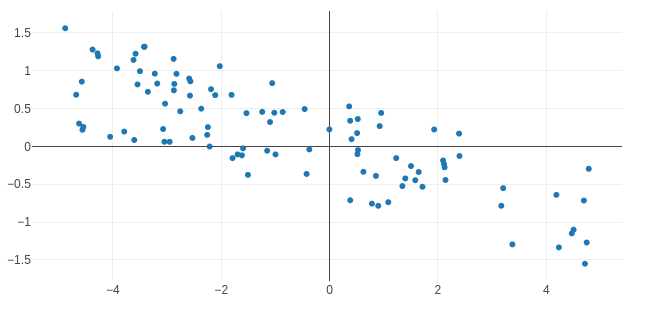
\includegraphics[width=0.49\textwidth]{correlation}
        \item 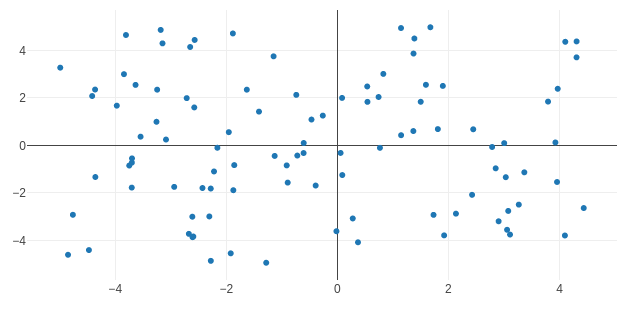
\includegraphics[width=0.49\textwidth]{nocorrelation}
    \end{enumerate}

\subsection{}

    Use the least squares method to provide a formula for the line of best fit $y = a + bx$ through the data below. The formula for the least squares method is reproduced below to help you.

    \begin{multicols}{2}
    $$ b = \frac{\sum{(x_i - \overline{x})(y_i - \overline{y})}}{\sum{(x_i - \overline{x})^2}} $$
    $$ a = \overline{y} - b\overline{x}$$
    \begin{center}
        \begin{tabular}{c | c}
            \toprule
            X & Y  \\
            \midrule
            1 & 5 \\
            2 & 7 \\
            3 & 10 \\
            4 & 9 \\
            \bottomrule
        \end{tabular}        
    \end{center}
\end{multicols}

\clearpage
\section{Probability}

\subsection{}

    You have 3 fair six-sided dice. What is the probability of

    \begin{enumerate}
        \item Rolling 3 sixes
        \item Rolling at least 2 sixes
    \end{enumerate}

\subsection{}

    Let $P(A) = 0.25$, $P(B) = 0.5$, and $P(C) = 0.75$. You know that events B and C are independant, and that $P(A \mid B ) = 0.7 $. Calculate the following

    \begin{enumerate}
        \item $P(A \cap B)$
        \item $P(B \cup A)$
        \item $P(B \cup C)$
    \end{enumerate}

\subsection{}

    Calculate the following

    \begin{multicols}{2}
        \begin{enumerate}
            \item $ 4! $
            \item $ 0! $
            \item $ ^4P_3 $
            \item $ ^{34}P_{23} $
            \item $ ^{11}C_{11} $
            \item $ ^{15}C_{7} $
        \end{enumerate}
    \end{multicols}

\subsection{}

    \begin{enumerate}
        \item How many combinations of four 8-bit binary numbers are possible?
        \item I define an ordering over the set \{a, b, c, d\}. How many possible orderings can I define?
    \end{enumerate}

\subsection{}

    $A_1$, and $A_2$ partition a probability space. $B_1, B_2,$ and $B_3$ partition the event $A_1$

    There is an event C, such that $P(C) = \frac{1}{2}$, and $P(C \mid A_2) = 0$
    
    There is an event D with 4 outcomes in $B_1$, 3 outcomes in $B_2$, and 0 outcomes in $B_3$. You know that $P (D \mid A_1 = \frac{1}{4})$

    \begin{enumerate}
        \item What is $\sum_{i=1}^3 P(C \mid B_i) $ ?
        \item What is $P(D \mid A_2)$
    \end{enumerate}
    
\subsection{}

    You have 3 bags of balls that each contain 80 balls, their colours are described in the table below.

    \begin{table}[h!]
        \centering
        \begin{tabular}{c | c | c }
            \toprule
            Bag & Red Balls & Black Balls \\
            \midrule
            Bag 1 & 65 & 15  \\
            Bag 2 & 23 & 57  \\
            Bag 3 & 23 & 57 \\
            \bottomrule
        \end{tabular}
    \end{table}

    You pick a bag at random and pick a random ball from that bag. What is the probability that you pick a red ball?

\subsection{}

    What is the liklihood that a student who passed their exam attended lectures?

    \begin{itemize}
        \item 80\% of students attend lectures
        \item 80\% of students pass their exam
        \item Of those who attend lectures, 95\% pass their exam
    \end{itemize}
    
\subsection{}

    You have 3 hypotheses that are disjoint and collectively exhaustive, $H_1, H_2, H_3$. The prior probability of each being true, and conditional probabilities that each is true given the event $E$ are given in the table below.

    \begin{table}[h!]
        \centering
        \begin{tabular}{c | c | c }
            \toprule
            $H_n$ & $P(H_n)$ & $P(E \mid H_n)$ \\
            \midrule
            $H_1$ & ${1}/{4}$ & ${3}/{4}$  \\
            $H_2$ & ${1}/{3}$ & ${1}/{2}$  \\
            $H_3$ & ${1}/{8}$ & ${2}/{7}$ \\
            \bottomrule
        \end{tabular}
    \end{table}

    Calculate posterior probabilities for all three hypotheses, given event E has been observed.


\clearpage
\section{Inferrential Statistics}

\subsection{}

The binomial distribution is given by 

\begin{center}
    $P(X = x) = ^nC_x.p^x.(1-p)^{(n-x)}$
\end{center}

Let X be a binomially distributed variable, with $n=6$ and $p=0.2$

\begin{enumerate}
    \item What is $P(X=2)$?
    \item What is the most likely value of X?
    \item What is $\sum_{i=1}^n P(X = i)$?
\end{enumerate}

\subsection{}

Let Y be a continuous variable uniformly distributed between 0 and 1.

\begin{enumerate}
    \item What is $P(Y = 0.5)$?
    \item What is $P(Y > 0.5)$?
\end{enumerate}

\subsection{}

Assuming a conventional experiment-wise value for $ \alpha = 0.05 $, and the Bonferroni adjustment for multiple testing ( $\alpha_{adjusted} = \frac{\alpha}{m}$), which of the experiments below report at least 1 statistically significant result.

\begin{enumerate}
    \item $ p = 0.04 $
    \item $ p = 0.12 $
    \item An experiment with two hypotheses, $p = 0.03$ and $p=0.04 $
    \item An experiment with three hypotheses, $p = 0.01$ $p=0.24$ and $p=0.0025 $ 
\end{enumerate}

\subsection{}

You run a series of experiments. The test statistics and degrees of freedom (if appropriate) are given below. For each, state whether the result is significant with $\alpha = 0.05$

\begin{enumerate}
    \item $z = 0.24 $
    \item $z = 2.1 $
    \item $t = 0.04$, $df = 33$
    \item $t = 4.31$, $df = 8$
\end{enumerate}

\subsection{}

I sample means of groups of size $n = 10$, with a mean of $\mu = 0$ and a standard deviation $\sigma = 2$. I get 0.4.

Calculate the z score

\subsection{}

You want to compare an observed difference between group means against an expected difference of 0. What do you use?

\begin{enumerate}
    \item Z test
    \item One sample t-test
    \item Paired t-test
    \item Two sample t-test
\end{enumerate}

\subsection{}

You take 5 friends to two ice cream shops. You get them to rate each shop out of 10. The data is given below.

\begin{table}[h!]
    \centering
    \begin{tabular}{c | c | c }
        \toprule
        Name & Shop A & Shop B \\
        \midrule
        John & 2 & 8  \\
        Mary & 3 & 8  \\
        Bill & 4 & 10 \\
        Sue & 2 & 10 \\
        Lisa & 1 & 7 \\
        \bottomrule
    \end{tabular}
\end{table}

What is the t statistic for the hypothesis that people prefer Shop B to Shop A?

\iffalse
\clearpage

$$ \sum_{i=1}^{n} i^2 = \frac{n(n+1)(2n + 1)}{6} $$

$$ \sum_{i=1}^{n} i $$

$$ \sum_{i=1}^{n} i = \frac{n(n + 1)}{2} $$

$$ \sum_{i=1}^{n} A_i = \frac{n(A_1 + A_n)}{2} $$

$$ \sum_{i=1}^{n} G_i = \frac{G_1(r^n - 1)}{r -1} $$


$$ A = \{ 10, 20, 30, 40 \}$$
$$ \sum_{i=1}^{4} A_i = 100$$
$$ \sum_i A_i = 100$$
$$ \sum A = 100$$

$$ \sum_{i=1}^{100} i = \frac{100(1 + 100)}{2} = 5050$$






$$ \sum_{i=1}^{n} ci = c \sum_{i=1}^{n} i $$

$$ \sum_{i=1}^{n} (a + b) = \sum_{i=1}^{n} a + \sum_{i=1}^{n} b $$

\begin{enumerate}
    \item $ \sum_{i=1}^{n} 2 $

    \item $ \sum_{i=1}^{n} a $

    \item $ \sum_{i=4}^{n} 10 $

    \item $ \sum_{i=0}^{n-1} (a + 4) $

    \item $ \sum_{i=-5}^{n+3} 13k^n$
\end{enumerate}

\begin{enumerate}
    \item $ \sum_{i=1}^{10} 1 $

    \item $ \sum_{i=1}^{10} i $

    \item $ \sum_{i=1}^{5} a $

    \item $ \sum_{i=1}^{10} i^2 $
\end{enumerate}




$ S_n = \frac{a(r^n - 1)}{r-1}$

$$ \prod_{i=1}^{n} a $$

$$ \prod_{k=1}^{n} c = c^n $$

\begin{enumerate}
    \item $ \prod_{k=1}^{4} 2 $

    \item $ \prod_{k=1}^{4} k $
    
    \item $ \prod_{k=1}^{3} \frac{k}{k+1} $

    \item $ \prod_{k=0}^{7} 2^k $
\end{enumerate}


\begin{enumerate}
    \item $ \sum_{i=1}^{n} 3ci $

    \item $ \sum_{i=1}^{n} (3i + 4) $

    \item $ \sum_{i=1}^{n} (2i^2 + 3i) $
\end{enumerate}

$$ \{a_1, a_2, \cdots, a_n, a_{n+1}, \cdots \} $$

$$ \{ a_n \} $$

$$ \{ a_n \}_{n=1}^{\infty} $$

\begin{enumerate}
    \item $ \{ n^2 + 3 \}_{n=1}^{\infty} $
    \item $ \{ \frac{n}{n+1} \}_{n=1}^{\infty} $
    \item $ \{ n + 3 \}_{n=4}^{17} $
    \item $ \{ k + \frac{n}{2} \}_{n=k}^{k+4} $
\end{enumerate}
\fi

\end{document}
